% Provenance (never printed): see sources/outline_sources.md (Year 1:
% observational astronomy, photometry). Telescopes, angular resolution,
% gratings, the Doppler effect and the black-body laws are owned by the
% physics series and recalled here. Curves computed in
% figdata/bachelor-1/{blackbody_bands, extinction_line}.py; numbers of the
% exercises and problem in the Book 3 scratch calculator ch02.py.
\chapter{望远镜、探测器与测光}\label{ch:b1:observing-the-sky}

天文学对恒星的全部认识，除了少数陨石
以及从月球和小行星取回的样品，都来自恒星发出的光。
这束光穿过地球大气，大气吸收了若干波段，
并模糊了其余部分；它被一面镜子收集，
镜子的大小既限制了能探测的最暗天体，
也限制了能分辨的最细节；它被探测器计数，
探测器把光子转化为电子，每一次计数都带有统计不确定度。
在亮度变为\omterm{def:b1:observing-the-sky:flux}{光度}或距离之前，上述每一步都必须被理解并加以修正。
本章沿着光从恒星到数值的路径展开：大气的窗口与消光定律，
望远镜与\omterm{def:b1:observing-the-sky:seeing}{视宁度}，探测器及其噪声，然后是星等、视差和颜色，
它们把测得的通量转化为恒星的性质。
同一层大气从下方看，是气候各章
（见\cref{ch:b1:radiation-heat-transport}）的研究对象；同样的测光方法用于行星，
则引出下一章
（见\cref{ch:b1:comparative-planetology}）。

\begin{recall}
望远镜的物镜在其口径上收集光线，并在焦点处成像；口径为 $D$ 的孔径
的衍射，把它能分辨的最小角度限制在约 $1.22\,\lambda/D$，
即瑞利判据（见物理系列本科一年级分册）。
衍射光栅按波长色散光（见本科二年级）；沿视线方向运动的光源，其谱线会因
多普勒效应而移动（见十二年级）。处于热平衡的物体辐射黑体谱，
其峰值服从维恩位移定律（见本科二年级）。在化学中，
溶液的吸\omterm{def:b1:observing-the-sky:flux}{光度}
与光程长度成正比。
\end{recall}

\section{大气窗口}

大气对某些波长是透明的，对另一些波长则是不透明的。
辐射主要被水蒸气、二氧化碳和臭氧吸收，
在最短的波长上，
则被高层大气中的原子和分子本身吸收。
% ledger: nasa:ems-absorbers

\begin{definition}[大气窗口]\label{def:b1:observing-the-sky:window}
称\emph{大气窗口}\index{大气窗口}为一段
波长范围，在该范围内，大气透过了自其顶部
直达地面的大部分辐射。\emph{光学窗口}自近紫外
延伸到近红外；\emph{射电窗口}自
约 1 厘米波长延伸到约 10 米波长。
\end{definition}

下图示意了大气对各波段的不透明度，
从伽马射线直至长波无线电波。伽马射线、X 射线以及
紫外线（波长短于约 \qty{0.3}{\micro\metre}）都到不了地面：
它们只能从太空观测。可见光能穿过大气，但会有一定模糊。大部分
红外辐射被水蒸气和二氧化碳吸收，只有
少数狭窄的窗口可供高\omterm{def:b1:spherical-astronomy:horizontal}{海拔}、干燥地点的地面天文台利用；近红外\omterm{def:b1:observing-the-sky:magnitude}{测光波段}
正位于其中，分别在 \qty{1.24}{\micro\metre}、
\qty{1.65}{\micro\metre} 和 \qty{2.16}{\micro\metre} 处。约
\qty{30}{\micro\metre} 至 1 毫米的波长再次被阻挡；
几厘米至约 10 米的无线电波可以穿过，甚至能穿过云层；更长的波则
被电离层反射。
% ledger: nasa:opacity-windows, baldry:2mass-pivot

\begin{omfigure}
\begin{tikzpicture}[x=1.0cm, y=2.2cm, font=\scriptsize]
% x = log10(lambda / 1 m) + 10 ; opacity 0..1 (schematic, after the NASA figure)
\fill[omSea!20] (0,0) rectangle (13,1.05);
\fill[brown!50] (0,0) -- (0,1) -- (3.45,1) -- (3.52,0.05) -- (4.03,0.05)
  -- (4.06,0.6) -- (4.09,0.15) -- (4.15,0.6) -- (4.22,0.15) -- (4.28,0.6)
  -- (4.34,0.15) -- (4.42,0.7) -- (4.55,0.25) -- (4.65,0.8) -- (4.9,0.2)
  -- (5.12,0.2) -- (5.25,0.7) -- (5.4,1) -- (7.0,1) -- (7.3,0.6) -- (7.6,0.75)
  -- (8.0,0.5) -- (8.5,0.03) -- (11.0,0.03) -- (11.3,1) -- (13,1) -- (13,0)
  -- cycle;
\draw[black!70] (0,0) rectangle (13,1.05);
\foreach \x in {0,...,13} { \draw (\x,0) -- (\x,-0.05); }
\foreach \x/\l in {0/0.1 nm, 2/10 nm, 4/1 \unit{\micro m}, 6/100 \unit{\micro m}, 8/1 cm,
  10/1 m, 12/100 m}
  { \node[below] at (\x,-0.05) {\l}; }
\foreach \y/\l in {0/0, 0.5/50, 1/100}
  { \draw (0,\y) -- (-0.1,\y); \node[left] at (-0.1,\y) {\l}; }
\node[rotate=90] at (-0.75,0.5) {不透明度（\%）};
\node at (6.5,-0.42) {\small 波长（对数刻度）};
\node[align=center] at (1.7,0.75) {伽马射线、X 射线、\\ 紫外线};
\node[align=center] at (6.2,0.75) {远红外};
\node[align=center] at (9.75,0.5) {射电窗口};
\node[omThm] at (4.15,0.86) {J H K};
\draw[-{Stealth}] (2.6,1.25) node[above] {光学窗口} -- (3.75,1.07);
\draw[-{Stealth}] (5.9,1.25) node[above] {红外窗口} -- (4.6,1.07);
\end{tikzpicture}

{\small 大气对来自太空的辐射的不透明度，
从 \qty{0.1}{nm} 到 \qty{1}{km}（对数刻度）。示意图，依据一幅
公有领域的 NASA 图件绘制：此处只关心窗口，而非
每个吸收带的确切形状。J、H、K 标示近红外\omterm{def:b1:observing-the-sky:magnitude}{测光波段}。}
% ledger: nasa:opacity-windows, nasa:ems-absorbers, baldry:2mass-pivot
\end{omfigure}

\subsection*{消光}

即使在光学窗口之内，大气仍会移除一部分光，
其方式包括吸收，以及被分子和气溶胶散射。沿光线方向，厚度为
$\mathrm ds$ 的薄层移除的强度比例
与 $\mathrm ds$ 成正比：$\mathrm dI = -\kappa I\,\mathrm ds$，其中
消光系数 $\kappa$（单位为每米）依赖于
波长以及该高度处空气的成分。这正是
溶液吸\omterm{def:b1:observing-the-sky:flux}{光度}定律在空气柱上的应用。

\begin{proposition}[布格定律]\label{prop:b1:observing-the-sky:bouguer}
沿穿过吸收介质的光线，强度按下式衰减：
\[
  I = I_0\,e^{-\tau}, \qquad \tau = \int_0^s \kappa\,\mathrm ds' ,
\]
其中 $I_0$ 为进入介质时的强度，$\tau$ 为
路径的光学厚度，是一个纯数。
对平面平行大气，\omterm{def:b1:spherical-astronomy:celestial-sphere}{天顶}距为 $z$（即恒星方向与竖直方向的夹角）的恒星，
其光线所经过的光学厚度为
$\tau(z) = \tau_0\sec z$，其中 $\tau_0$ 为
\omterm{def:b1:spherical-astronomy:celestial-sphere}{天顶}处的光学厚度。
\end{proposition}

\begin{proof}
方程 $\mathrm dI/I = -\kappa\,\mathrm ds$ 可分离变量，自
大气顶（$I = I_0$，$s = 0$）积分到观测者处，得
$\ln(I/I_0) = -\int_0^s\kappa\,\mathrm ds'$。在平面平行大气中
$\kappa$ 仅依赖于高度 $y$，而与竖直方向夹角为 $z$ 的光线
其行进 $\mathrm ds = \mathrm dy/\cos z$ 的路程，即爬升 $\mathrm dy$。由此
可得 $\tau(z) = \int \kappa(y)\,\mathrm dy/\cos z = \tau_0\sec z$。
\end{proof}

\begin{definition}[大气质量，大气消光系数]\label{def:b1:observing-the-sky:extinction}
观测的\emph{大气质量}\index{大气质量} $X$ 为视线的光学厚度
与\omterm{def:b1:spherical-astronomy:celestial-sphere}{天顶}处光学厚度之比：
$X = \tau(z)/\tau_0$。\omterm{def:b1:spherical-astronomy:celestial-sphere}{天顶}处其值为 1，对平面平行的
大气，$X = \sec z$。某一波段的
\emph{大气消光系数}\index{大气消光系数} $k$ 是
经过一个大气质量所造成的以星等计的变暗量。因此，
大气顶之上星等为 $m_0$ 的恒星，其观测星等为
\[
  m = m_0 + kX .
\]
\end{definition}

星等的定义见\cref{sec:b1:observing-the-sky:magnitudes}；这里只需用到：
因子 $e^{-\tau}$ 造成的变暗相当于增加
$2.5\log_{10}e\;\tau = 1.086\,\tau$ 星等，因而 $k = 1.086\,\tau_0$。
平面平行近似下的\omterm{def:b1:observing-the-sky:extinction}{大气质量}在高度角低至约
\ang{30}（$X = 2$）时仍十分准确，在地平线附近则失效，此时 $\sec z$ 无限增大，
而弯曲大气中的真实路径长度仍为有限值；
因此观测者避免在低高度角观测，这既出于此原因，也为避开随路径增长而加剧的
模糊。

\begin{method}[消光直线]\label{met:b1:observing-the-sky:extinction-line}
求恒星在大气顶之上的星等 $m_0$：
\begin{enumerate}
  \item 于一夜之中，随恒星升起或落下，
        在若干个\omterm{def:b1:observing-the-sky:extinction}{大气质量}下测量该恒星或某颗标准星的星等 $m$；
  \item 由\omterm{def:b1:spherical-astronomy:celestial-sphere}{天顶}距计算每个\omterm{def:b1:observing-the-sky:extinction}{大气质量}，$X = \sec z$；
  \item 以 $m$ 对 $X$ 作图，并用最小二乘法拟合一条直线；
  \item 斜率即为该夜该波段的
        消光系数 $k$；$X = 0$ 处的截距即为 $m_0$。
\end{enumerate}
同一夜中，该波段内观测的其他恒星均可用同一个
$k$ 作修正：$m_0 = m - kX$。
\end{method}

\begin{example}
某夜，在 V 波段对一颗恒星测量了六次：
\begin{center}
\small
\begin{tabular}{lcccccc}
\hline
$X$ & 1.05 & 1.18 & 1.36 & 1.62 & 1.95 & 2.31 \\
$m$ & 8.024 & 8.031 & 8.072 & 8.104 & 8.171 & 8.216 \\
\hline
\end{tabular}
\end{center}
下图所示的最小二乘直线，
斜率为 $k = \qty{0.160}{\mag}$ 每\omterm{def:b1:observing-the-sky:extinction}{大气质量}，截距为 $m_0 = 7.851$。
各点绕该直线的散布为 \num{0.006} 星等，
这正是一个好夜晚的测光精度。在\omterm{def:b1:spherical-astronomy:celestial-sphere}{天顶}处，恒星因消光变暗 \num{0.16}
星等，因而损失了 $1 - 10^{-0.4\times0.160} = \qty{14}{\percent}$ 的
光量。
\end{example}

\begin{omfigure}
\begin{tikzpicture}
\begin{axis}[omrecord, width=0.62\linewidth, height=5.4cm, xmin=0, xmax=2.5,
  ymin=7.80, ymax=8.28, y dir=reverse, xlabel={大气质量 $X$},
  ylabel={星等 $m$}, yticklabel style={/pgf/number format/fixed,
  /pgf/number format/precision=2}, tick label style={font=\scriptsize},
  label style={font=\small}]
\addplot[omThm, line width=0.9pt, dashed] table[x=X, y=m] {figdata/out/bachelor-1-extinction_line-fit.dat};
\addplot[only marks, mark=*, mark size=1.6pt, omDef] table[x=X, y=m] {figdata/out/bachelor-1-extinction_line-obs.dat};
\node[font=\scriptsize, right, fill=white, inner sep=1pt] at (axis cs:0.05,7.83) {$m_0 = 7.851$};
\node[font=\scriptsize, fill=white, inner sep=1pt, rotate=-10] at (axis cs:0.95,8.10) {斜率 $k = 0.160$};
\end{axis}
\end{tikzpicture}

{\small 消光直线：一颗恒星在六个\omterm{def:b1:observing-the-sky:extinction}{大气质量}下的星等
（圆点）及最小二乘直线，外推至 $X = 0$ 处，
即大气顶之上的星等。星等向下增大：越暗的恒星位置越
低。}
\end{omfigure}

\subsection*{视宁度}

望远镜上方的空气从不静止。温度略有差异、因而折射率也略有差异的
空气团漂移穿过光束，使其产生微小的随机偏折，
且每秒变化许多次。
肉眼看到恒星闪烁；长时间曝光所记录的
则是一个模糊光斑，比望远镜的衍射图样大得多。

\begin{definition}[视宁度]\label{def:b1:observing-the-sky:seeing}
某台址的\emph{视宁度}\index{视宁度}，是点源经大气湍流
在长时间曝光中模糊后所成像的角直径，
以像的半高全宽度量，
单位为角秒。
\end{definition}

\omterm{def:b1:observing-the-sky:seeing}{视宁度}随夜而变，也随时而变。台址正是据此选定的：
在\omterm{def:b1:spherical-astronomy:horizontal}{海拔} \qty{4204}{m} 的毛纳基山顶，
自由大气\omterm{def:b1:observing-the-sky:seeing}{视宁度}的中位数约为 \ang{;;0.40}，冬季约为 \ang{;;0.45}，
夏季为 \ang{;;0.35}，最好的十分之一夜晚的\omterm{def:b1:observing-the-sky:seeing}{视宁度}低于
约 \ang{;;0.25}；同一台址上空
的可降水汽量中位数仅为 \qty{0.9}{mm}，这使其红外窗口得以开放。
% ledger: cfht:site, cfht:seeing

\section{望远镜与分辨率}

望远镜有两个作用：一是在物镜的面积上收集光，
并成像使细节得以分辨。
收集面积随 $D^2$ 增长：口径为两倍的镜面，
在相同时间内收集到四倍的光子，能探测到暗四倍的恒星。
分辨率受衍射限制，约为 $1.22\,\lambda/D$，
同时还受\omterm{def:b1:observing-the-sky:seeing}{视宁度}的限制。

\begin{example}
加拿大–法国–夏威夷望远镜位于莫纳克亚山，口径为
\qty{3.58}{m}。在 \qty{550}{nm} 波长下，其衍射极限为
\[
  1.22\times\frac{\qty{550e-9}{m}}{\qty{3.58}{m}} = \qty{1.87e-7}{rad}
  = \ang{;;0.039},
\]
比同一地点的中值\omterm{def:b1:observing-the-sky:seeing}{视宁度} \ang{;;0.40} 精细十倍。两种极限
在口径 $D = 1.22\lambda/\theta =
1.22\times\qty{550e-9}{m}/(\num{0.40}/\num{206265}) = \qty{0.35}{m}$ 时相等：任何
宽于约 \qty{35}{cm} 的地基望远镜，在可见光波段都受\omterm{def:b1:observing-the-sky:seeing}{视宁度}限制，
而非其自身光学系统。
% ledger: cfht:aperture, cfht:seeing
\end{example}

因此，大型地基望远镜增加的是集光面积，而非清晰度，
除非它能校正湍流。\emph{自适应光学}正是为此而设：
传感器每秒多次测量来自亮星
（或由高层大气中激光器制造的人造星）的波前如何被扭曲，
并由许多小型致动器弯曲一面薄镜面，以抵消这种扭曲。校正在
红外波段效果最好，因为那里的湍流更慢、更弱，
且适用于导星附近的小视场。
在太空中则完全没有\omterm{def:b1:observing-the-sky:seeing}{视宁度}。

\section{探测器}

眼睛在极短的时间内积累光线，只对进入其中的
光子中很小一部分作出响应。照相底片可积分数小时，
但只记录了光的很小一部分。现代天文学使用
由半导体制成的光子探测器，其中每个吸收了足够能量的光子
都会释放一个电子。

\begin{definition}[量子效率，信噪比]\label{def:b1:observing-the-sky:detector}
探测器在给定波长下的\emph{量子效率}\index{量子效率} $\eta$，
是其记录为光电子的入射光子所占的比例：
$\eta = N_\mathrm{e}/N_\gamma$。测量的
\emph{信噪比}\index{信噪比}是测得信号
除以其标准差，
即其随机误差的典型大小。
\end{definition}

\emph{电荷耦合器件}（CCD）是光学窗口的标准探测器。
它是一块被划分为像素网格的薄硅片，
每个像素都是一个势阱，用于储存曝光期间在其中被吸收的光子所释放的电子。
曝光结束后，依次加在电极上的电压将电荷逐像素、逐行移动，
送至单个放大器逐个测量，图像即为计数表。
CCD 在可见光的大部分波段上记录了入射光子的很大一部分，
其响应与所接收的光量成正比，直到每个像素达到最大电荷量
（其\emph{满阱容量}）为止，并且可以积分数小时。
红外阵列采用相同原理，
只是使用其他半导体材料，
并逐像素读出。

光子的到达是随机的。若某光源在一次曝光中平均产生 $N$ 个光电子，
则实际记录的计数在相邻曝光之间，
以标准差 $\sqrt N$ 涨落（泊松统计，
在本阶段不加证明地承认：稀有独立事件的计数）。

\begin{proposition}[光子噪声]\label{prop:b1:observing-the-sky:snr}
当仅来自光源的光子噪声占主导时，每秒产生 $R$ 个光电子的光源
在时间 $t$ 内测得的
\omterm{def:b1:observing-the-sky:detector}{信噪比}为
\[
  \mathrm{SNR} = \frac{Rt}{\sqrt{Rt}} = \sqrt{Rt} ;
\]
它随曝光时间的平方根增长，并随望远镜口径增长
（因为 $R \propto D^2$）。星等的误差则为
$\sigma_m \approx 1.086/\mathrm{SNR}$。
\end{proposition}

\begin{proof}
信号为 $N = Rt$，其标准差为 $\sqrt N$。对于星等，
$m = -2.5\log_{10}N + \text{常数}$，因此微小误差 $\sigma_N$
给出 $\sigma_m = 2.5\log_{10}e\;\sigma_N/N = 1.086/\mathrm{SNR}$。
\end{proof}

要将星等测量到 \num{0.01}，需要\omterm{def:b1:observing-the-sky:detector}{信噪比}约为 109，即
约 \num{12000} 个光电子。对于暗弱光源，还有另外两项需要考虑。
天空本身会发光，星像的每个像素也会以
速率 $B$ 收集天空光子；放大器还会为每次读出的像素引入读出噪声 $\sigma_r$。
完整的表达式为
\[
  \mathrm{SNR} = \frac{Rt}{\sqrt{Rt + Bt + n\sigma_r^2}}
\]
其中 $n$ 为图像所含像素数。对于亮星，它简化为 $\sqrt{Rt}$，
对于比天空更暗的光源，它简化为 $R\sqrt t/\sqrt B$。由于 $B$ 随
视宁盘面积增大，良好的\omterm{def:b1:observing-the-sky:seeing}{视宁度}带来双重好处：图像更清晰，既能分辨更多细节，
又收集到更少的天空光（\cref{exo:b1:observing-the-sky:11}）。

\begin{inthefield}[夜晚的望远镜]
测光工作对定标与对星体的观测同样依赖。夜晚开始前，
专业天文台的观测者要拍摄\emph{本底}图像
（零曝光时长，记录每个像素的电子偏置）和
\emph{平场}图像（圆顶内部均匀照明或晨昏天空的成像，
用以描绘灵敏度如何在各像素之间变化，
乃至在整个视场内变化）；科学图像通过减去本底
并除以平场进行校正。夜间，对已知星等的标准星在
多个\omterm{def:b1:observing-the-sky:extinction}{大气质量}下进行观测，以确定消光直线和
将计数转换为星等的零点。该夜称为
\emph{测光夜}，即消光在此修正期间足够稳定；
在莫纳克亚山顶，\qty{55}{\percent} 的
夜晚为测光夜。
% ledger: cfht:nights
\begin{center}
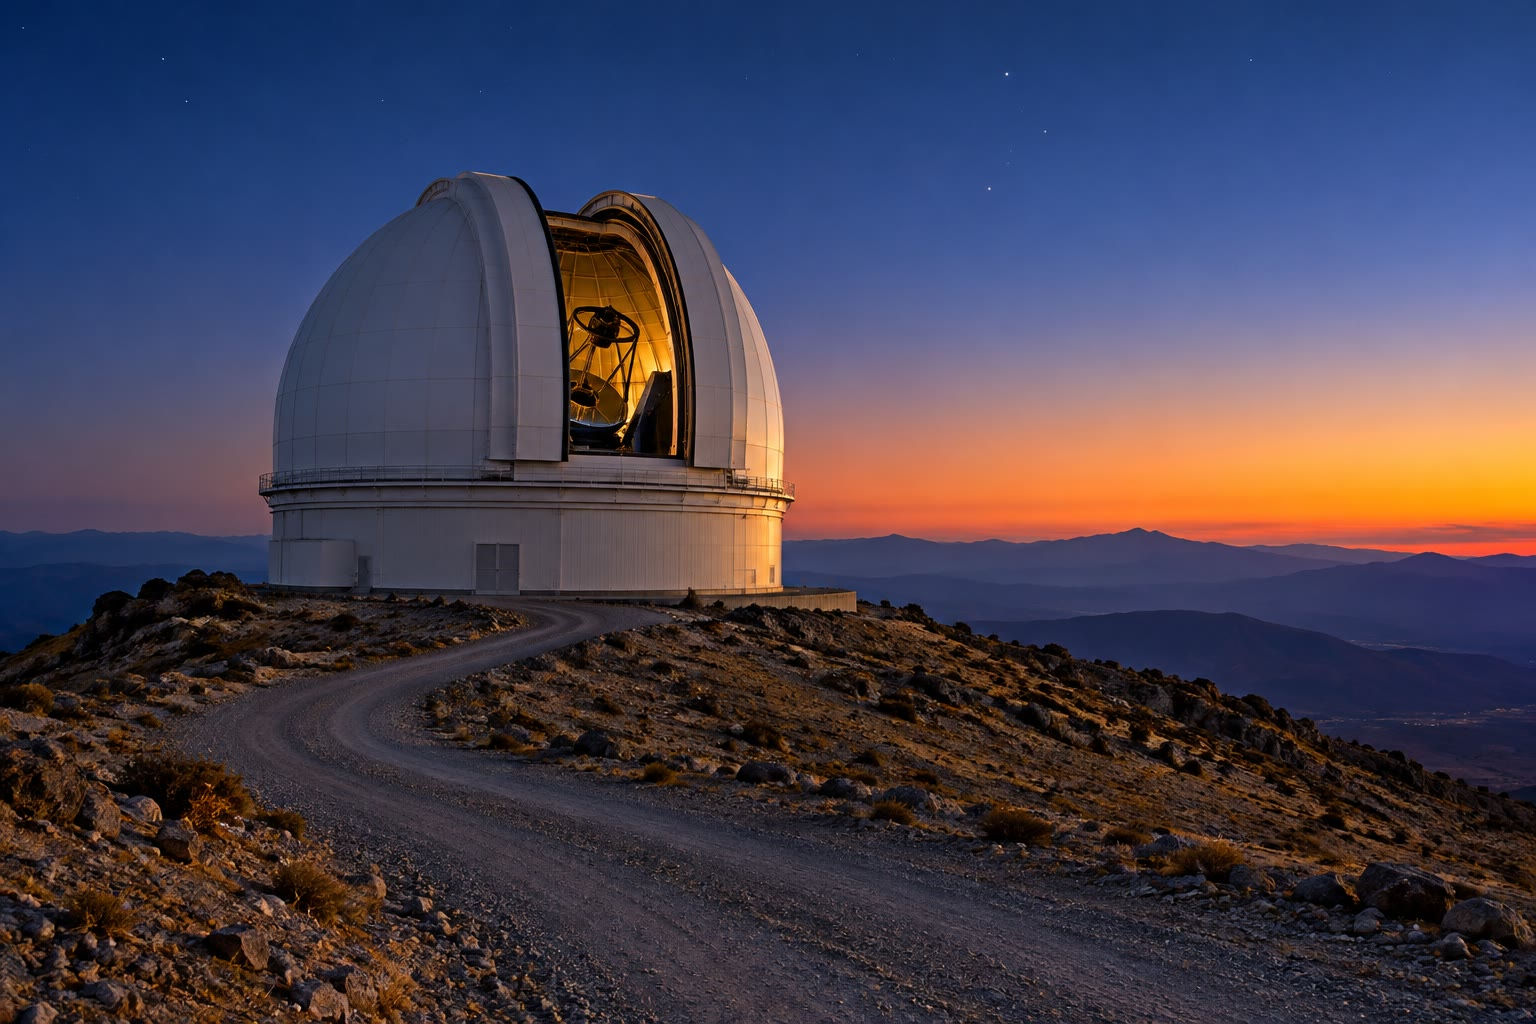
\includegraphics[width=0.55\linewidth]{images/book3/ai/b1-observatory-dusk.jpg}
\end{center}
\end{inthefield}

\section{通量与星等}\label{sec:b1:observing-the-sky:magnitudes}

\begin{definition}[流量，光度]\label{def:b1:observing-the-sky:flux}
来自某源的\emph{流量}\index{流量（源的）} $F$ 是该源辐射
穿过一个与其方向垂直的单位面积的功率，单位为瓦特每平方米；
若限制在某一波长范围内，则为该波段内的流量。该源的
\emph{光度}\index{光度} $L$ 是其辐射的
总功率，单位为瓦特。
\end{definition}

\begin{proposition}[平方反比律]\label{prop:b1:observing-the-sky:inverse-square}
\omterm{def:b1:observing-the-sky:flux}{光度}为 $L$、向各方向均匀辐射的源，
在真空中距离为 $d$ 处，其\omterm{def:b1:observing-the-sky:flux}{流量}为
\[
  F = \frac{L}{4\pi d^2} .
\]
\end{proposition}

\begin{proof}
在无吸收的稳态下，由能量守恒，穿过以该源为中心的任一球面的功率
都等于 $L$。由对称性，它
均匀分布在该球面的面积 $4\pi d^2$ 上。
\end{proof}

\begin{example}
太阳的\omterm{def:b1:observing-the-sky:flux}{光度}为 \qty{3.828e26}{W}。在一个天文单位
\qty{1.496e11}{m} 处，其\omterm{def:b1:observing-the-sky:flux}{流量}为 $\num{3.828e26}/(4\pi\times
(\num{1.496e11})^2) = \qty{1361}{W.m^{-2}}$：这就是地球
在大气层顶所接收到的太阳辐照度。
% ledger: sun:L, const:au, earth:TSI
\end{example}

\omterm{def:b1:observing-the-sky:flux}{流量}的变化范围极大，天文学家采用
一种对数标度来比较它们，该标度沿用自肉眼可见恒星曾被划分的类别：
最亮的属于一等，
最暗的属于六等。

\begin{definition}[视星等，测光波段]\label{def:b1:observing-the-sky:magnitude}
\emph{测光波段}\index{测光波段}是一段波长范围，
由标准滤光片选出，以字母命名：U（紫外）、B（蓝）、
V（视觉）、R（红）、I（近红外），以及红外窗口中的 J、H、K。
源在某一波段中的\emph{视星等}\index{视星等} $m$
由其在该波段中的\omterm{def:b1:observing-the-sky:flux}{流量} $F$ 定义为
\[
  m_1 - m_2 = -2.5\log_{10}\frac{F_1}{F_2} ,
\]
零点由标准星确定，
各波段中约等于织女星的星等。星等相差 5 等，
\omterm{def:b1:observing-the-sky:flux}{流量}恰好相差 100 倍；相差 1 等，则\omterm{def:b1:observing-the-sky:flux}{流量}之比为 $100^{1/5} = 2.512$。越亮的
源，星等越小，且可能为负值。
\end{definition}

标准 U、B、V、R、I 滤光片的枢轴波长分别为
\qty{358.5}{nm}、\qty{437.1}{nm}、\qty{547.8}{nm}、\qty{650.4}{nm} 和
\qty{802.0}{nm}。
% ledger: baldry:bessell-pivot
在 V 波段，太阳的\omterm{def:b1:observing-the-sky:magnitude}{视星等}为 $-26.74$，夜空中最亮的恒星天狼星为
$-1.46$，织女星为 $0.03$。因此太阳
在我们的天空中比天狼星亮 $10^{0.4\times(26.74 - 1.46)} = \num{1.29e10}$ 倍；
但这尚不能说明二者谁更亮，
这还需要知道距离。
% ledger: nasa:sun-V, simbad:sirius, simbad:vega

\subsection*{周年视差与秒差距}

地球绕太阳运行时，一颗近处的恒星相对于
远得多的背景恒星似乎在移动，一年中描出一个小椭圆。这
种视运动是测量恒星距离最直接的方法：它
以地球轨道作为测量基线。

\begin{definition}[周年视差，秒差距]\label{def:b1:observing-the-sky:parallax}
恒星的\emph{周年视差}\index{周年视差} $p$ 是
在恒星处由地球轨道半径（即一个天文单位）所张的角，
并从与视线垂直的方向观察；它是
恒星在一年中所描出的椭圆的半长轴。
\emph{秒差距}\index{秒差距}（\unit{\parsec}）是一个天文单位
恰好张开一角秒时的距离：
\[
  \qty{1}{\parsec} = \frac{\qty{1}{\au}}{\tan\ang{;;1}} = \qty{206265}{\au}
  = \qty{3.0857e16}{m} = \qty{3.2616}{\lightyear} .
\]
\end{definition}

由于 $p$ 极小，$\tan p \approx p$，单位为弧度，
距离随即可得：
\[
  d = \frac{\qty{1}{\au}}{\tan p} \quad\Longrightarrow\quad
  \frac{d}{\unit{\parsec}} = \frac{1}{p/\text{角秒}} .
\]
天狼星的视差为 \ang{;;0.37921}，因此其距离为 $1/0.37921 =
\qty{2.637}{\parsec}$，即 \qty{8.60}{\lightyear}。即使是最近的恒星
视差都小于一角秒，小于\omterm{def:b1:observing-the-sky:seeing}{视宁度}：视差是由
恒星像中心的位移求得的，大量光子能
比像的宽度精确得多地确定其位置。本章末尾
所述的一项空间任务已用这种方法测定了
近二十亿个天体的位置。
% ledger: simbad:sirius, const:au, esa:gaia

\begin{omfigure}
\begin{tikzpicture}[font=\small]
\draw[black!50] (0,0) ellipse (2.0cm and 0.55cm);
\fill[orange!80!black] (0,0) circle (3pt) node[below=3pt] {太阳};
\fill[blue!70!black] (-2.0,0) circle (2pt) node[left, align=right] {地球，\\六个月后};
\fill[blue!70!black] (2.0,0) circle (2pt) node[right] {地球};
\fill (0,4.4) circle (1.6pt) node[above] {恒星};
\draw[omDef, thick] (0,0) -- node[right, pos=0.55] {$d$} (0,4.4);
\draw[omThm] (2.0,0) -- (0,4.4);
\draw[omThm, dashed] (-2.0,0) -- (0,4.4);
\draw[thick] (0,0) -- node[above] {\qty{1}{\au}} (2.0,0);
\draw[omThm] (0,3.75) arc[start angle=-90, end angle=-65.6, radius=0.65cm];
\node[omThm] at (0.17,3.38) {$p$};
\end{tikzpicture}

{\small \omterm{def:b1:observing-the-sky:parallax}{周年视差}（未按比例）：从恒星处看去，地球轨道半径
所张的角为 $p$。相隔六个月时，恒星的方向相差
$2p$。最近恒星的真实角度小于
一角秒。}
\end{omfigure}

\begin{definition}[绝对星等，距离模数]\label{def:b1:observing-the-sky:absolute}
称恒星在某一波段的\emph{绝对星等}\index{绝对星等}为 $M$，它是该星
在距离为
\qty{10}{\parsec}处、在真空中观测所得的\omterm{def:b1:observing-the-sky:magnitude}{视星等}。差 $m - M$ 称为其
\emph{距离模数}\index{距离模数}。
\end{definition}

\begin{proposition}[距离模数]\label{prop:b1:observing-the-sky:modulus}
设恒星位于距离 $d$ 处，并在真空中观测，则
\[
  m - M = 5\log_{10}\frac{d}{\qty{10}{\parsec}} .
\]
若光在途中被减弱了 $A$ 个星等的消光，
则 $m - M = 5\log_{10}(d/\qty{10}{\parsec}) + A$。在某一波段内，两颗恒星的
\omterm{def:b1:observing-the-sky:flux}{光度}之比为 $L_1/L_2 = 10^{0.4(M_2 - M_1)}$。
\end{proposition}

\begin{proof}
由平方反比律，距离 $d$ 处与 \qty{10}{\parsec}处的\omterm{def:b1:observing-the-sky:flux}{流量}
之比为 $F(d)/F(\qty{10}{\parsec}) = (\qty{10}{\parsec}/d)^2$。由
星等的定义给出 $m - M = -2.5\log_{10}(\qty{10}{\parsec}/d)^2
= 5\log_{10}(d/\qty{10}{\parsec})$。消光使\omterm{def:b1:observing-the-sky:flux}{流量}乘以
$10^{-0.4A}$，相当于将 $A$ 加到 $m$ 上。在共同距离
\qty{10}{\parsec}处，两星的\omterm{def:b1:observing-the-sky:flux}{流量}之比等于\omterm{def:b1:observing-the-sky:flux}{光度}之比，并且
$M_1 - M_2 = -2.5\log_{10}(L_1/L_2)$。
\end{proof}

太阳的\omterm{def:b1:observing-the-sky:absolute}{绝对星等}为 $M_\odot = 4.83$，\omterm{def:b1:observing-the-sky:flux}{光度}为
\qty{3.828e26}{W}。将恒星的 V 波段\omterm{def:b1:observing-the-sky:absolute}{绝对星等}与
太阳的相比，即得其 V 波段以太阳\omterm{def:b1:observing-the-sky:flux}{光度}为单位的\omterm{def:b1:observing-the-sky:flux}{光度}，
$L/L_\odot = 10^{0.4(4.83 - M)}$——这是\emph{V 波段\omterm{def:b1:observing-the-sky:flux}{光度}}，因为
温度与太阳相差很大的恒星，其功率中
位于 V 波段之外的份额并不相同。
% ledger: sun:Mabs, sun:L

\subsection*{颜色}

\begin{definition}[色指数]\label{def:b1:observing-the-sky:colour-index}
恒星的\emph{色指数}\index{色指数}是其在两个波段的星等之差，
先列较蓝的波段，最常用的是 $B - V$。
$B - V$ 小或为负表示蓝色恒星，大则为红色恒星。
\end{definition}

\omterm{def:b1:observing-the-sky:colour-index}{色指数}与距离无关，因为平方反比律使两个波段同等地变暗；
它度量的是光谱的形状，因而可反映
恒星表面的温度。恒星的辐射大致与黑体辐射相同，
其光谱峰值位于 $\lambda_\mathrm{max} = b/T$（维恩位移定律，
$b = \qty{2.898e-3}{m.K}$，取自物理系列的本科二年级分册）。
下图画出了三条黑体光谱：一个
温度为 \qty{3500}{K} 的冷体，峰值位于近红外，
其 V 波段的\omterm{def:b1:observing-the-sky:flux}{流量}大于 B 波段；太阳的有效温度 \qty{5772}{K}，峰值位于
\qty{502}{nm}，介于 B 与 V 之间；温度为 \qty{10000}{K} 的天体峰值位于
紫外，其 B 波段比 V 波段更亮。B 与 V 的辐射度之比随温度升高而稳定增大，
三条曲线对应的数值依次为 \num{0.46}、\num{0.97} 和
\num{1.53}，这正是 $B - V$ 随 $T$ 升高而减小的原因。
% ledger: const:b, nasa:sun-Teff, baldry:bessell-pivot

\begin{omfigure}
\begin{tikzpicture}
\begin{axis}[omrecord, width=0.9\linewidth, height=5.8cm, xmin=200, xmax=1500,
  ymin=0, ymax=1.17, xtick={200,400,...,1400}, ytick={0,0.5,1},
  xlabel={波长 (nm)},
  ylabel={$B_\lambda$ / 最大值}, tick label style={font=\scriptsize},
  label style={font=\small}, legend style={font=\scriptsize, at={(0.5,1.03)},
  anchor=south, draw=none, fill=none}, legend columns=3]
\addplot[red!75!black, line width=1.1pt] table[x=lam_nm, y=t3500] {figdata/out/bachelor-1-blackbody_bands-curves.dat};
\addplot[orange!90!black, line width=1.1pt] table[x=lam_nm, y=t5772] {figdata/out/bachelor-1-blackbody_bands-curves.dat};
\addplot[omDef, line width=1.1pt] table[x=lam_nm, y=t10000] {figdata/out/bachelor-1-blackbody_bands-curves.dat};
\legend{\qty{3500}{K}, \qty{5772}{K}（太阳）, \qty{10000}{K}}
\draw[black!45, densely dashed] (axis cs:358.5,0) -- (axis cs:358.5,1.06);
\node[font=\scriptsize, above, inner sep=1pt] at (axis cs:358.5,1.06) {U};
\draw[black!45, densely dashed] (axis cs:437.1,0) -- (axis cs:437.1,1.06);
\node[font=\scriptsize, above, inner sep=1pt] at (axis cs:437.1,1.06) {B};
\draw[black!45, densely dashed] (axis cs:547.8,0) -- (axis cs:547.8,1.06);
\node[font=\scriptsize, above, inner sep=1pt] at (axis cs:547.8,1.06) {V};
\draw[black!45, densely dashed] (axis cs:650.4,0) -- (axis cs:650.4,1.06);
\node[font=\scriptsize, above, inner sep=1pt] at (axis cs:650.4,1.06) {R};
\draw[black!45, densely dashed] (axis cs:802.0,0) -- (axis cs:802.0,1.06);
\node[font=\scriptsize, above, inner sep=1pt] at (axis cs:802.0,1.06) {I};
\end{axis}
\end{tikzpicture}

{\small 三种温度下的黑体光谱，各除以各自的最大值，
并标出 U、B、V、R、I 各滤光片的枢轴波长（虚线）。
峰值随温度升高向短波方向移动（维恩
位移定律）：\qty{828}{nm}、\qty{502}{nm} 和 \qty{290}{nm}。}
% ledger: const:h, const:c, const:kB, const:b, nasa:sun-Teff, baldry:bessell-pivot
\end{omfigure}

四颗亮星展示了颜色的范围：
\begin{center}
\small
\begin{tabular}{lcccc}
\hline
恒星 & $V$ & $B$ & $B - V$ & 视差（\unit{mas}）\\
\hline
参宿七 & 0.13 & 0.10 & $-0.03$ & 3.78 \\
河鼓二 & 0.76 & 0.98 & 0.22 & 194.95 \\
北极星 & 2.02 & 2.62 & 0.60 & 7.54 \\
参宿四 & 0.42 & 2.27 & 1.85 & 6.55 \\
\hline
\end{tabular}
\end{center}
% ledger: simbad:rigel, simbad:altair, simbad:polaris, simbad:betelgeuse
参宿七呈蓝白色，参宿四与之同属一个星座，呈橙红色：一种
肉眼可见的颜色差异。二者的
光谱型 B8 与 M1--M2 用光谱的语言说明了同样的差异，
而光谱学正是本科三年级分册的主题。

\section{光谱仪}

测光在若干较宽的波段中测量光；光谱仪则把光展开
成光谱。来自望远镜焦点的光穿过一条狭窄的
狭缝，经准直器变为平行光，再经光栅（或棱镜）色散，
最后由照相机聚焦到探测器上，每个波长落在
像素的不同列上
（见下图）。刻线数为 $N$ 的光栅，
被照亮部分在第 $k$ 级使用时，可分辨相距
$\Delta\lambda$ 的两个波长，条件为 $\lambda/\Delta\lambda \le kN$，其
分辨率（回顾物理系列本科二年级分册）。

\begin{omfigure}
\begin{tikzpicture}[font=\scriptsize, >=Stealth]
\draw[thick, fill=omSea!25] (0.15,0) ellipse (0.13 and 0.9);
\node[below] at (0.15,-0.95) {物镜};
\draw[omDef] (-1.3,0.75) -- (0.15,0.75) -- (2.4,0);
\draw[omDef] (-1.3,-0.75) -- (0.15,-0.75) -- (2.4,0);
\draw[omDef, ->] (-1.3,0) -- (-0.2,0);
\node[above] at (-0.8,0.75) {星光};
\draw[very thick] (2.4,-0.35) -- (2.4,-0.06); \draw[very thick] (2.4,0.06) -- (2.4,0.35);
\node[above] at (2.4,0.38) {狭缝};
\draw[omDef] (2.4,0) -- (3.6,0.55); \draw[omDef] (2.4,0) -- (3.6,-0.55);
\draw[thick, fill=omSea!25] (3.6,0) ellipse (0.1 and 0.72); \node[below] at (3.6,-0.74) {准直器};
\draw[omDef] (3.6,0.55) -- (4.9,0.55); \draw[omDef] (3.6,-0.55) -- (4.9,-0.55);
\draw[thick, pattern=north east lines] (4.85,-0.8) rectangle (5.0,0.8);
\node[below] at (4.92,-0.82) {光栅};
\draw[blue!70!black] (5.0,0.3) -- (6.4,0.95); \draw[red!70!black] (5.0,0.3) -- (6.4,-0.15);
\draw[blue!70!black] (5.0,-0.3) -- (6.4,0.35); \draw[red!70!black] (5.0,-0.3) -- (6.4,-0.75);
\draw[thick, fill=omSea!25] (6.4,0.1) ellipse (0.1 and 1.08); \node[below] at (6.4,-1.0) {照相机};
\draw[blue!70!black] (6.4,0.95) -- (7.6,0.55); \draw[blue!70!black] (6.4,0.35) -- (7.6,0.55);
\draw[red!70!black] (6.4,-0.15) -- (7.6,-0.45); \draw[red!70!black] (6.4,-0.75) -- (7.6,-0.45);
\fill[black!70] (7.6,-0.8) rectangle (7.75,0.9);
\node[right, align=left] at (7.8,0.05) {探测器：\\ 每列一个 \\ 波长};
\end{tikzpicture}

{\small 光穿过望远镜与光栅光谱仪的光路
（示意图，望远镜物镜与光学元件以透镜表示，
图中示出两个波长）：狭缝截取恒星的像，准直器使光束变为平行光，
光栅将其色散，照相机
将每个波长聚焦到探测器上各自的位置。}
\end{omfigure}

光谱包含三类信息。其\emph{谱线}在恒星大气中原子与离子吸收处呈暗线，
在热而稀薄的气体发射处呈亮线，
可用来确定所含的化学元素。其连续谱的形状，
以及在不同温度下形成的谱线的相对强度，
给出气体的温度。而谱线的多普勒位移
给出视线方向上的速度：静止波长为 $\lambda$ 的谱线，
位移为 $\Delta\lambda = \lambda v_r/c$，径向速度 $v_r$
远小于 $c$。测量 $v_r$ 精确到 \qty{1}{km.s^{-1}} 需要
的分辨率约为 $c/v_r = \num{300000}$，或用中等分辨率
配合同时测量的大量谱线。光谱如何揭示恒星与星系的结构、
组成与运动，
是本科三年级分册的主题。

\section{从太空观测}

大气层之上没有封闭的窗口，没有消光，没有\omterm{def:b1:observing-the-sky:seeing}{视宁度}问题，
红外波段也没有温暖空气的辐射。空间望远镜为此付出了代价：
成本高昂，质量与尺寸受火箭运载能力限制，
且其中大多数无法维修。它们用于地面无法胜任的场合：
伽马射线、X 射线和紫外线，它们永远到达不了地面；
红外波段中超出狭窄窗口的部分；
宽视场下达到衍射极限的图像；
以及一些测量，例如极多恒星的视差，
这些测量需要稳定的仪器，并置于湍流大气之外。

\begin{dated}{2026}
% ledger: nasa:hubble-mirror, nasa:jwst-mirror, nasa:jwst-orbit, nasa:jwst-launch, nasa:jwst-range, esa:gaia
三台空间天文台可以展示这一范围。哈勃空间望远镜
于 1990 年发射，主镜口径为 \qty{2.4}{m}。詹姆斯·韦伯空间望远镜
于 2021 年 12 月 25 日发射，主镜口径为 \qty{6.5}{m}，由
18 块六边形子镜拼成，集光面积为 \qty{25}{m^2}；其工作波长范围为
\qty{0.6}{\micro\metre} 至 \qty{28.5}{\micro\metre}，绕太阳运行，
位于日地系统第二拉格朗日点 L2 附近，距地球 150 万千米，
在背离太阳的一侧。
盖亚于 2013 年 12 月 19 日发射至同一区域，使用两台望远镜，
二者共用一个 CCD 焦平面，以三维方式测绘近 20 亿个天体的位置与运动；
其观测已经结束，
星表正在陆续发布。
\end{dated}

\begin{omfigure}
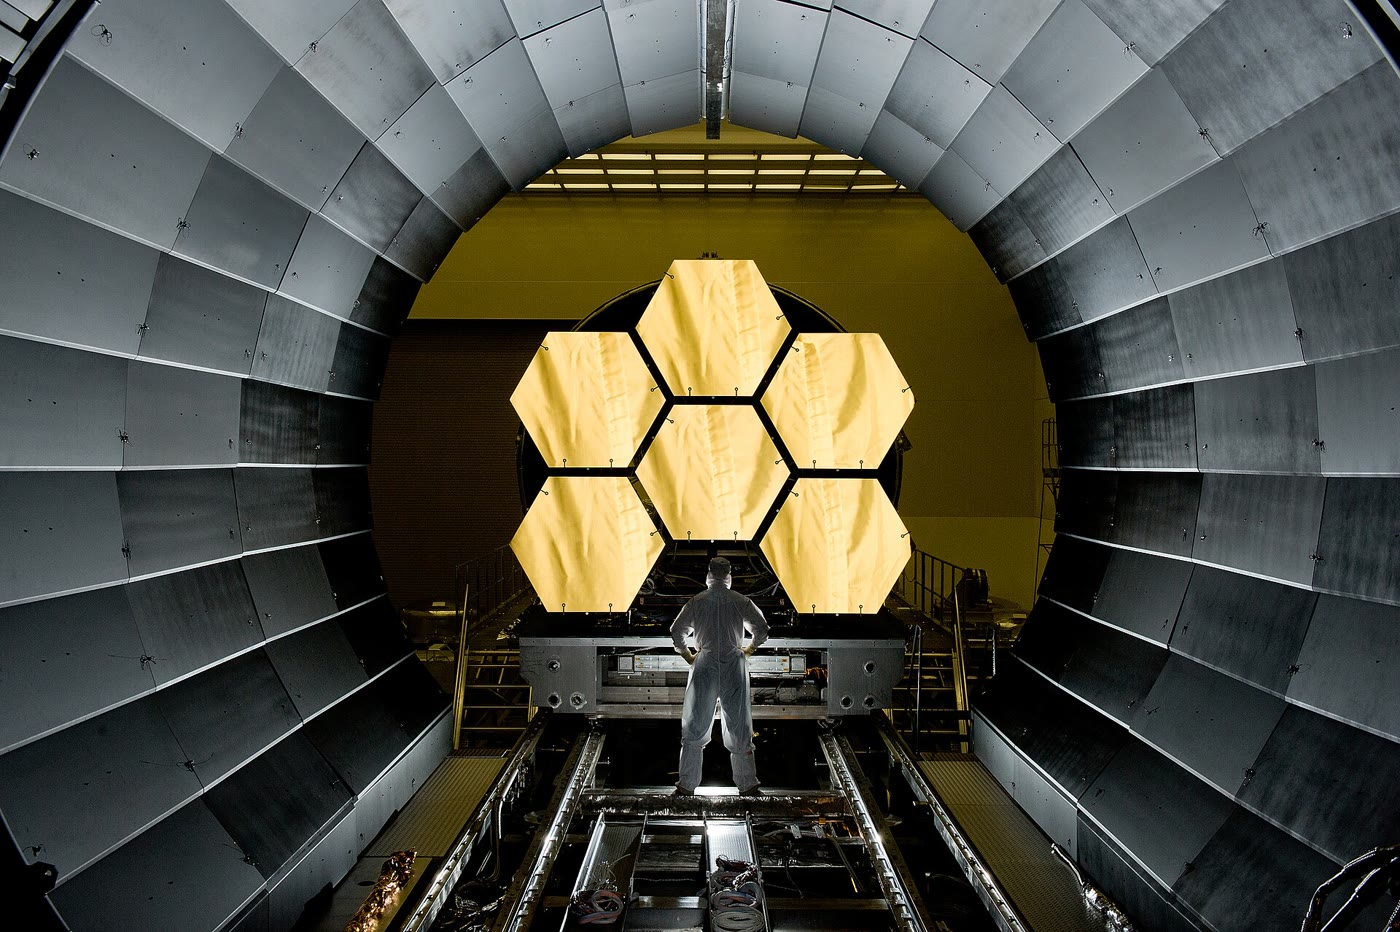
\includegraphics[width=0.78\linewidth]{images/book3/b1-jwst-mirror-segments.jpg}

{\small 詹姆斯·韦伯空间望远镜主镜 18 块六边形子镜中的六块，
2011 年准备进行低温测试；18 块子镜在太空中展开后，
共同构成宽 \qty{6.5}{m} 的镜面。照片：NASA/MSFC/David Higginbotham，
公有领域。}
% ledger: commons:jwst-mirror, nasa:jwst-mirror
\end{omfigure}

\section{练习}

\begin{exercise}[$\star$]\label{exo:b1:observing-the-sky:1}
求星等分别为 1.0 与 6.0 的两颗恒星的通量之比，
以及参宿七（$V = 0.13$）与北极星（$V = 2.02$）的通量之比，并判断天空中哪一颗更亮。
\end{exercise}

\begin{exercise}[$\star$]\label{exo:b1:observing-the-sky:2}
河鼓二的视差为 \ang{;;0.19495}。求其距离，以\omterm{def:b1:observing-the-sky:parallax}{秒差距}、
天文单位和光年表示。
\end{exercise}

\begin{exercise}[$\star$]\label{exo:b1:observing-the-sky:3}
计算口径为 \qty{2.4}{m} 的空间望远镜在
\qty{550}{nm} 处的衍射极限（以角秒计），并与\omterm{def:b1:observing-the-sky:seeing}{视宁度}
\ang{;;0.40} 相比较。再对口径为 \qty{6.5}{m} 的望远镜在
\qty{2.0}{\micro\metre} 处做同样的计算。
\end{exercise}

\begin{exercise}[$\star$]\label{exo:b1:observing-the-sky:4}
根据四颗亮星的表，将参宿七、牵牛星、勾陈一和
参宿四按表面温度从高到低排序。为什么在距离相差很大的恒星之间，
可以比较它们的\omterm{def:b1:observing-the-sky:colour-index}{色指数}？
\end{exercise}

\begin{exercise}[$\star\star$]\label{exo:b1:observing-the-sky:5}
某恒星在同一夜间，\omterm{def:b1:spherical-astronomy:celestial-sphere}{天顶}距为 \ang{30} 时测得星等为 6.412，
在\omterm{def:b1:spherical-astronomy:celestial-sphere}{天顶}距为 \ang{60} 时测得星等为 6.590。假设大气为平行平面大气，
计算两次观测的\omterm{def:b1:observing-the-sky:extinction}{大气质量}、消光系数以及
该恒星在大气层外的星等。
\end{exercise}

\begin{exercise}[$\star\star$]\label{exo:b1:observing-the-sky:6}
某恒星在 \qty{10}{s} 的曝光中产生 400 个光电子，
且仅由恒星自身的光子噪声占主导。求其\omterm{def:b1:observing-the-sky:detector}{信噪比}。要使\omterm{def:b1:observing-the-sky:detector}{信噪比}达到 100，
需曝光多长时间？要使星等的测量不确定度达到
\num{0.01}，又需曝光多长时间？
\end{exercise}

\begin{exercise}[$\star\star$]\label{exo:b1:observing-the-sky:7}
参宿七的 $V = 0.13$，视差为 \ang{;;0.00378}。忽略
其与地球之间的消光，计算其距离、\omterm{def:b1:observing-the-sky:absolute}{绝对星等}，
以及以太阳单位表示的 V 波段\omterm{def:b1:observing-the-sky:flux}{光度}（$M_\odot = 4.83$）。
\end{exercise}

\begin{exercise}[$\star\star$]\label{exo:b1:observing-the-sky:8}
比较口径为 \qty{2.4}{m} 的圆形镜面（忽略其
中心遮挡）与韦伯望远镜（\qty{25}{m^2}）的集光面积。韦伯望远镜收集相同数目光子所需的
曝光时间缩短了多少？
其集光面积占口径为 \qty{6.5}{m} 的整个圆盘面积的
比例是多少？为什么该比例小于一？
\end{exercise}

\begin{exercise}[$\star\star$]\label{exo:b1:observing-the-sky:9}
(a) 由太阳的\omterm{def:b1:observing-the-sky:flux}{光度} \qty{3.828e26}{W}，计算其在
\qty{10}{\parsec} 处的\omterm{def:b1:observing-the-sky:flux}{流量}。(b) 太阳的\omterm{def:b1:observing-the-sky:magnitude}{视星等}和\omterm{def:b1:observing-the-sky:absolute}{绝对星等}分别为
$-26.74$ 和 $4.83$。利用\omterm{def:b1:observing-the-sky:absolute}{距离模数}求出日地距离，
以天文单位表示。
\end{exercise}

\begin{exercise}[$\star\star\star$]\label{exo:b1:observing-the-sky:10}
由\cref{prop:b1:observing-the-sky:bouguer}证明：$k =
2.5\log_{10}e\;\tau_0$。对于消光线之夜（$k =
\num{0.160}$），计算\omterm{def:b1:spherical-astronomy:celestial-sphere}{天顶}光学厚度 $\tau_0$，以及
在\omterm{def:b1:spherical-astronomy:celestial-sphere}{天顶}和 $X = 2.31$ 处到达望远镜的光所占的比例。
若采用平行平面大气，在\omterm{def:b1:spherical-astronomy:celestial-sphere}{天顶}距
为 \ang{85} 处的\omterm{def:b1:observing-the-sky:extinction}{大气质量}会给出什么预测？为什么不应相信该数值？
\end{exercise}

\begin{exercise}[$\star\star\star$]\label{exo:b1:observing-the-sky:11}
一颗暗弱的星系在望远镜中每秒给出 $R = 50$ 个光电子，
其像所在区域内的天空每秒给出 $B = \num{2000}$ 个光电子，当
\omterm{def:b1:observing-the-sky:seeing}{视宁度}为 \ang{;;0.80} 时。读出噪声可忽略。(a) 要使\omterm{def:b1:observing-the-sky:detector}{信噪比}达到 10，
需曝光多长时间？(b) 天空在像上的贡献随视宁圆盘的面积而增长。
对\omterm{def:b1:observing-the-sky:seeing}{视宁度}为 \ang{;;0.40} 的情形重复上述计算。(c) 证明：对于比天空暗弱得多的源，
给定\omterm{def:b1:observing-the-sky:detector}{信噪比}所需的曝光时间
与 $\theta^2/D^2$ 成正比，其中 $\theta$ 为\omterm{def:b1:observing-the-sky:seeing}{视宁度}，$D$ 为
望远镜的口径。
\end{exercise}

\begin{exercise}[$\star\star\star$]\label{exo:b1:observing-the-sky:12}
一块每毫米 1200 条线的光栅，照明宽度为 \qty{100}{mm}，
使用一级光谱。(a) 其分辨本领是多少，以及
在 \qty{550}{nm} 处能分辨的最小波长差是多少？(b) 该波长差
对应多大的径向速度？(c) 地球绕太阳运动的
速度为 \qty{29.78}{km.s^{-1}}。这一运动能使一条位于
\qty{550}{nm} 处的谱线移动多少？相当于多少个分辨元？
因此，测量恒星视向速度的观测者必须怎样做？
% ledger: earth:vorb
\end{exercise}

\section{问题：称一称天狼星的光}

\begin{problem}[{周末问题——天狼星有多远、看上去有多亮，
发出多少光子，以及它的亮度相当于多少个太阳}]
\label{pb:b1:observing-the-sky:1}
% ledger: simbad:sirius, simbad:vega, simbad:sirius-b, nasa:sun-V, sun:Mabs, const:au
% numbers computed in the scratch calculator calc/ch02.py from the rounded data
天狼星是夜空中最亮的恒星，它有一颗暗弱的伴星，
即白矮星天狼星~B。利用下列数据：
\begin{center}
\small
\begin{tabular}{lcc}
\hline
天体 & $V$ & 视差 \\
\hline
天狼星 & $-1.46$ & \ang{;;0.37921} \\
天狼星 B & $8.44$ &——\\
织女星 & $0.03$ & \ang{;;0.13023} \\
太阳 & $-26.74$ &——\\
\hline
\end{tabular}
\end{center}
其中 $M_\odot = 4.83$（V 波段），$\qty{1}{\parsec} = \qty{206265}{\au} =
\qty{3.0857e16}{m} = \qty{3.2616}{\lightyear}$，观测台处的
消光系数为每个\omterm{def:b1:observing-the-sky:extinction}{大气质量} $k = 0.15$。

\medskip
\noindent\textbf{第一部分——天狼星有多远？}
\begin{enumerate}
  \item 计算天狼星的距离，以\omterm{def:b1:observing-the-sky:parallax}{秒差距}表示。
  \item 以天文单位和米表示该距离。
  \item 以光年表示该距离。我们今夜所见的光
        是多久以前离开天狼星的？
  \item 一年之内，天狼星的方向左右摆动的总角度
        是多少？将其与\omterm{def:b1:observing-the-sky:seeing}{视宁度} \ang{;;0.40} 相比较。
        为什么这一摆动仍能测得\omterm{def:b1:observing-the-sky:seeing}{视宁度}的
        很小一部分？
  \item 若视差误差为 \ang{;;0.001}，距离的相对误差
        是多少？由此引起的距离误差相当于多少光年？
\end{enumerate}

\medskip
\noindent\textbf{第二部分——它看起来有多亮？}
\begin{enumerate}[resume]
  \item 计算天狼星与织女星在 V 波段的通量之比。
  \item 计算太阳与天狼星的通量之比。
  \item 计算天狼星与天狼星~B 的通量之比。
  \item 在帕拉纳尔天文台，天狼星经过子午线时的
        高度为 \ang{82.09}（见\cref{ch:b1:spherical-astronomy}）。计算
        该时刻的\omterm{def:b1:observing-the-sky:extinction}{大气质量}、消光量与
        所测得的星等。
  \item 在高度 \ang{30} 处重复上述计算。光在
        传播途中损失了多大比例？
  \item 为什么公式 $X = \sec z$ 会误导
        用于测量刚升起后的天狼星的观测者？
\end{enumerate}

\medskip
\noindent\textbf{第三部分——光子计数。}
一台安装在 \qty{1}{m} 望远镜上的照相机，每秒记录 $\num{3.0e4}$ 个光电子，
对象为星等 $V = 10.0$ 的恒星，已改正消光。
每个像元至多容纳 $\num{1.0e5}$ 个电子（即其满阱容量）。
\begin{enumerate}[resume]
  \item 照相机每秒从天狼星~B
        记录多少个光电子？
  \item 仅计入恒星自身的光子噪声，多长的曝光可使天狼星~B 的
        \omterm{def:b1:observing-the-sky:detector}{信噪比}达到 1000？此时其星等的误差为多少？
  \item 照相机每秒从天狼星
        记录多少个光电子？
  \item 若天狼星的光有 \qty{20}{\percent} 落在其最亮的
        像元中，该像元充满需要多长时间？
  \item 图像上，天狼星像的微弱翼部在天狼星~B 所在位置
        每像元沉积天狼星光的 $10^{-4}$，而天狼星~B 最亮的
        像元收集其自身光的 \qty{20}{\percent}。比较该像元中
        两者的速率。
  \item 不使该像元饱和的最长曝光时间是多少？
        计算该曝光时间内天狼星~B 在该像元中的\omterm{def:b1:observing-the-sky:detector}{信噪比}，
        \qty{0.5}{s}，并计入两个源的光子噪声。天狼星~B
        能否被探测到？是什么使其难以探测？
\end{enumerate}

\medskip
\noindent\textbf{第四部分——相当于多少个太阳？}
\begin{enumerate}[resume]
  \item 计算天狼星的\omterm{def:b1:observing-the-sky:absolute}{距离模数}。
  \item 推算天狼星在 V 波段的\omterm{def:b1:observing-the-sky:absolute}{绝对星等}，精确到小数点后两位。
  \item 计算织女星的距离与\omterm{def:b1:observing-the-sky:absolute}{绝对星等}。
  \item 天狼星与织女星中，哪一颗在 V 波段的本征\omterm{def:b1:observing-the-sky:flux}{光度}更高，
        并相差多少倍？
  \item 从天狼星的距离处看太阳，其\omterm{def:b1:observing-the-sky:magnitude}{视星等}
        将为多少？若取 6.0 为暗夜中肉眼可见的最暗星等，
        它是否可见？
  \item 天狼星在多远的距离上仍可被肉眼看到？
  \item 以太阳单位计算天狼星的 V 波段\omterm{def:b1:observing-the-sky:flux}{光度}：天狼星
        比多少个太阳还亮？
\end{enumerate}
\end{problem}
